\documentclass[aspectratio=169,10pt]{beamer}

\usetheme{Madrid}
\usecolortheme{whale}

\usepackage[T1]{fontenc}
\usepackage[utf8]{inputenc}
\usepackage{lmodern}
\usepackage{booktabs}
\usepackage{array}
\usepackage{tikz}
\usetikzlibrary{arrows.meta, positioning}

\setbeamertemplate{navigation symbols}{}
\setbeamertemplate{itemize items}[circle]

\setbeamercolor{block title}{bg=blue!70!black,fg=white}
\setbeamercolor{block body}{bg=blue!8,fg=black}

\setbeamercolor{alerted text}{fg=red!70!black}

\title[SAKLOLO]{SAKLOLO: A Hybrid Semantic-Probabilistic Framework for Analysing Social Media Emergency Feeds in Bulacan and CAMANAVA}

\subtitle{Undergraduate Research Proposal -- Title Defense}

\author[Group 10]{
	Mariel Alvarado \and
	Jaizel Dela Paz \and
	Juliana Rojimherie B. Jornal \and
	William James N. Landicho
}

\institute[BulSU]{
	Group 10 -- B.S. Mathematics -- Computer Science Specialization \\
	College of Science, Bulacan State University
}

\date{October 2026}

\begin{document}
	
	% =========================================================
	% TITLE
	% =========================================================
	\begin{frame}
		\titlepage
	\end{frame}
	
	
	% =========================================================
	% 1. PROBLEM
	% =========================================================
	\begin{frame}{Problem}
		
		\begin{itemize}
			\item Emergency social media feeds are high-volume, unstructured, and time-sensitive.
			\item Critical rescue, damage, and sentiment signals are buried in noisy Taglish posts.
			\item Manual monitoring is too slow for DRRMOs in Bulacan and CAMANAVA.
		\end{itemize}
		
	\end{frame}
	
	
	% =========================================================
	% 2. SOLUTION -- STUDY NAMIN
	% =========================================================
	\begin{frame}{Solution: SAKLOLO}
		
		\begin{columns}[T]
			
			\column{0.48\textwidth}
			
			\begin{block}{System A -- Hybrid baseline}
				\begin{itemize}
					\item Count Vectorization
					\item LDA topics
					\item XLM-RoBERTa sentiment
					\item Joint Matrix
				\end{itemize}
			\end{block}
			
			\column{0.48\textwidth}
			
			\begin{block}{System B -- LLM comparison}
				\begin{itemize}
					\item Qwen3-1.7B-Instruct-Q4\_K\_M
					\item Few-shot prompting
					\item Matched topic count
					\item Joint Matrix output
				\end{itemize}
			\end{block}
			
		\end{columns}
		
		\vspace{1mm}
		
		\begin{alertblock}{Main idea}
			Benchmark a lightweight interpretable hybrid system against a modern open-weight LLM on the same Taglish disaster corpus.
		\end{alertblock}
		
	\end{frame}
	
	
	% =========================================================
	% 3. SOP -- STATEMENT OF THE PROBLEM
	% =========================================================
	\begin{frame}{SOP: Statement of the Problem}
		
		\begin{enumerate}
			\item How does System B perform relative to System A in sentiment classification?
			\item How strongly are latent topics associated with sentiment in each system?
			\item Is there a significant operational difference between the outputs in blind stakeholder evaluation?
		\end{enumerate}
		
		\vspace{1mm}
		
		\begin{block}{Focus}
			Agreement, association, and usability -- not just accuracy.
		\end{block}
		
	\end{frame}
	
	
	% =========================================================
	% 4. SCOPE
	% =========================================================
	\begin{frame}{Scope}
		
		\begin{columns}[T]
			
			\column{0.48\textwidth}
			
			\textbf{Included}
			\begin{itemize}
				\item Public Facebook posts/comments
				\item Bulacan + CAMANAVA
				\item 2020--2025
				\item Tagalog, English, Taglish
				\item 10,000--15,000+ records
				\item Offline local dashboard
			\end{itemize}
			
			\column{0.48\textwidth}
			
			\textbf{Excluded}
			\begin{itemize}
				\item Real-time DRRM integration
				\item Private posts
				\item Cloud deployment
				\item Rescue dispatch simulation
				\item Enterprise multi-user system
			\end{itemize}
			
		\end{columns}
		
	\end{frame}
	
	
	% =========================================================
	% 5. SIGNIFICANCE
	% =========================================================
	\begin{frame}{Significance}
		
		\begin{itemize}
			\item \textbf{DRRMOs:} faster triage of emergency feeds.
			\item \textbf{LGUs:} localized sentiment and topic insights.
			\item \textbf{Responders:} organized field information.
			\item \textbf{Researchers:} benchmark for Taglish disaster NLP.
		\end{itemize}
		
		\vspace{1mm}
		
		\begin{block}{Value}
			SAKLOLO supports decision-making by converting chaotic social feeds into structured topic--sentiment evidence.
		\end{block}
		
	\end{frame}
	
	
	% =========================================================
	% 6. QUICK RRL
	% =========================================================
	\begin{frame}{Quick RRL}
		
		\begin{itemize}
			\item \textbf{Global:} LDA and transformer hybrids cluster disaster text in floods and typhoons.
			\item \textbf{Philippines:} Social media aids response and recovery, but noise and misinformation remain problems.
			\item \textbf{Local:} Philippine LDA studies exist, but mostly use formal posts, tweets, or non-emergency Taglish feeds.
			\item \textbf{BulSU:} Related theses focus on GPS, alerts, and location sharing, not NLP triage.
			\item \textbf{Gap:} No rigorous benchmark of hybrid joint matrix vs. open-weight LLM for Bulacan/CAMANAVA emergency feeds.
		\end{itemize}
		
	\end{frame}
	
	
	% =========================================================
	% 7. CONCEPTUAL FRAMEWORK
	% =========================================================
	\begin{frame}{Conceptual Framework}
		
		\begin{center}
			
			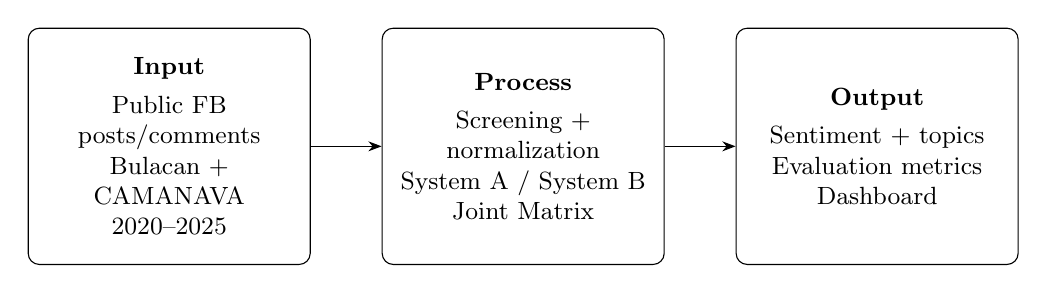
\begin{tikzpicture}[
				node distance=9mm,
				>=Stealth,
				box/.style={
					draw,
					rounded corners,
					align=center,
					inner sep=4pt,
					font=\small,
					text width=3.3cm,
					minimum size=3cm
				}
				]
				
				\node[box] (input) {
					\textbf{Input} \\[1mm]
					Public FB posts/comments \\
					Bulacan + CAMANAVA \\
					2020--2025
				};
				
				\node[box, right=of input] (process) {
					\textbf{Process} \\[1mm]
					Screening + normalization \\
					System A / System B \\
					Joint Matrix
				};
				
				\node[box, right=of process] (output) {
					\textbf{Output} \\[1mm]
					Sentiment + topics \\
					Evaluation metrics \\
					Dashboard
				};
				
				\draw[->] (input) -- (process);
				\draw[->] (process) -- (output);
				
			\end{tikzpicture}
			
		\end{center}
		
		\vspace{1mm}
		
		\begin{alertblock}{Logic}
			Same corpus $\rightarrow$ two systems $\rightarrow$ same matrix shape $\rightarrow$ fair comparison.
		\end{alertblock}
		
	\end{frame}
	
	
	% =========================================================
	% 8. RESEARCH METHOD
	% =========================================================
	\begin{frame}{Research Method}
		
		\begin{itemize}
			\item Comparative quantitative evaluation design.
			\item Same prepared corpus for System A and System B.
			\item System A is the relative reference; no absolute ground truth is claimed.
		\end{itemize}
		
		\vspace{-1mm}
		
		\begin{table}
			\centering
			\small
			\begin{tabular}{@{}lll@{}}
				\toprule
				RQ & Metrics & Threshold \\
				\midrule
				RQ1 & Precision, Recall, Macro-F1 & Macro-F1 $\geq 0.70$ \\
				RQ1 & Cohen's $\kappa$ & $\geq 0.60$ \\
				RQ2 & Chi-square, Cram\'er's V & $p < 0.05$, $V > 0.07$ \\
				RQ3 & Agreement rate, McNemar's test & $\geq 70\%$, $\alpha = 0.05$ \\
				\bottomrule
			\end{tabular}
		\end{table}
		
	\end{frame}
	
	
	% =========================================================
	% 9. SYSTEM DEVELOPMENT -- WATERFALL
	% =========================================================
	\begin{frame}{System Development: Waterfall}
		
		\begin{enumerate}
			\item \textbf{Requirements:} fix corpus, metrics, and output format.
			\item \textbf{Design:} define System A/B pipelines and dashboard.
			\item \textbf{Implementation:} build collection, preprocessing, models, and UI.
			\item \textbf{Testing:} run both systems, compute statistics, conduct blind evaluation.
			\item \textbf{Documentation:} report results, limitations, and handover materials.
		\end{enumerate}
		
		\vspace{1mm}
		
		\begin{block}{Why Waterfall?}
			The comparison rules are fixed before development to preserve validity.
		\end{block}
		
	\end{frame}
	
	
	% =========================================================
	% 10. RESPONDENTS
	% =========================================================
	\begin{frame}{Respondents}
		
		\begin{columns}[T]
			
			\column{0.48\textwidth}
			
			\textbf{Cohort A: DRRM officers}
			\begin{itemize}
				\item 5--10 active practitioners
				\item Bulacan/CAMANAVA offices
				\item Judge operational usefulness
			\end{itemize}
			
			\column{0.48\textwidth}
			
			\textbf{Cohort B: technical experts}
			\begin{itemize}
				\item 5--10 faculty/researchers
				\item Math, CS, data analytics
				\item Judge coherence and validity
			\end{itemize}
			
		\end{columns}
		
		\vspace{1mm}
		
		\begin{alertblock}{Blind panel}
			Total: 10--20 evaluators; outputs labeled only as X and Y.
		\end{alertblock}
		
	\end{frame}
	
	
	% =========================================================
	% 11. DATA GATHERING PROCEDURE
	% =========================================================
	\begin{frame}{Data Gathering Procedure}
		
		\begin{enumerate}
			\item Identify public disaster-related Facebook sources in Bulacan and CAMANAVA.
			\item Extract posts/comments using semi-automated scraping and manual screening.
			\item Apply inclusion/exclusion criteria.
			\item Normalize text, remove duplicates, and anonymize identifiers.
			\item Run the same corpus through System A and System B.
			\item Generate joint matrices and compute evaluation metrics.
			\item Present blinded outputs to the stakeholder panel through the dashboard.
		\end{enumerate}
		
	\end{frame}
	
	
	% =========================================================
	% 12. ETHICAL CONSIDERATION
	% =========================================================
	\begin{frame}{Ethical Consideration}
		
		\begin{itemize}
			\item Only publicly accessible posts/comments are collected.
			\item Personal identifiers and usernames are removed.
			\item Data handling follows RA 10173, the Data Privacy Act of 2012.
			\item Evaluators give voluntary participation and informed consent.
			\item Results are reported transparently for academic use only.
		\end{itemize}
		
	\end{frame}
	
	
	% =========================================================
	% CLOSING
	% =========================================================
	\begin{frame}
		\centering
		
		{\Large Thank You}\\[3mm]
		
		{\large Questions from the Panel}\\[2mm]
		
		\small
		SAKLOLO -- Group 10, Bulacan State University
		
	\end{frame}
	
\end{document}